\documentclass[a4paper,11pt]{article}
\usepackage[utf8]{inputenc}
\usepackage[english]{babel}
\usepackage{url} %url parsing
\usepackage[colorlinks, allcolors=blue]{hyperref} %advanced referencing options
\usepackage{float} %better images/tables positioning
\usepackage{graphicx} %better image insertion
\usepackage{amsmath} %text in equasions (include the 2 packages below)
\usepackage{amsfonts}
\usepackage{amssymb}
\usepackage{IEEEtrantools}
\usepackage{outlines} %sub-items in lists
\usepackage{fancyhdr}
\usepackage{csquotes} %more consistent quotes
\usepackage{comment}
\usepackage[backend=bibtex,bibencoding=utf8]{biblatex}
\usepackage[parfill]{parskip} %Sane paragraphs at last! The same can be acheived with the 2 lines below:
%\setlength{\parskip}{5pt}
%\setlength{\parindent}{0pt}
\usepackage{neuralnetwork}
\usepackage{caption}
\usepackage{tikz}
\usetikzlibrary{automata,positioning,shapes.geometric,fit}
\bibliography{mybib.bib}
\pagestyle{fancy}
\extramarks{\markboth}{}
%\lhead{\markboth}
\rhead{\thepage}
\begin{document}
\pagenumbering{gobble}
\thispagestyle{empty}
\title{Thesis Draft}
\author{Eugeio Maria Capuani}
\maketitle
\cleardoublepage
\pagenumbering{arabic}
\section{Introduction}
\subsection{Motivation}
The aim of this thesis is to evaluate the paper \enquote{PassGAN: A Deep Learning Approach for Password Guessing}\cite{PassGAN}, by testing the Deep Learning system described in the paper with a different dataset of leaked passwords from Italy\cite{libero_leak} (henceforth referred to as the Libero dataset), to test whether there are any differences in performance when PassGAN is used to crack a database from a non-english source.\newline

This dataset is composed of real user passwords belonging to the Italian email provider Libero.it, that were leaked in 2016. We believe the use of these passwords to be ethical because this particular leak has been public for a number of years. %And the company has since taken action to remediate?
\newline

The underlying tough behind this it to test whether differences in grammar and language have any noticeable effect when training the system: perhaps GANs are expressive enough that they 
can account for the different provenance of the data without any significant change, or maybe some adjustments should be made such as the inclusion of Natural Language corpora on the training data. One other possible change might be to mix password datasets from English and non-English sources.

The inclusion Natural language corpora might present its own challenges, such as the fact that some prior studies with GANs and RNNs indicates that the inclusion of such data ends up creating a lot of noise rather than improving performance\cite{PassGAN, Melicher2016}. %Check is PassGAN paper has such a claim.

These studies instead seem to suggest that one should "focus the network's effort" so to speak, by using data that is as close as possible to the desired result.\newline

One might make the case that linguistic differences are not that relevant when it comes to passwords, that the use of grammatical constructs is often trumped by patters of user behaviour in password creation that are international and well represented in rule-based password crackers. Thus, it should not matter where the network learns these patterns.

On the other hand, in our early attempts to train PassGAN on the Libero dataset we observed that most of the passwords the system generates attempt to mimic the sound and structure of Italian words; This leads us to speculate that the inclusion on natural language corpora might help the system to generate grammatically correct words, and thus perhaps improve performance.

Another interesting possibility could be the application of Transference Learning, which has proven useful in other cases such as \cite{Melicher2016}. By using Transference Learning to train on the Libero dataset and then on some natural language corpora, we might be able to nudge the system towards grammatically correct passwords without having to change the input data.\newline 
 
In conclusion, we believe this research might contribute some insight in the role that grammatical features have in password cracking, when this task is approached using Deep Neural Networks: many papers on the subject ask the question of whether Deep Learning systems are expressive enough to generate novel passwords and thus yield results that are not achievable with traditional password cracking methods, and we see this research as part of this ongoing quest into exploring the capabilities and limits of Deep Learning-based password crackers.

%\subsection{Problem formulation}

\cleardoublepage
%Talk more about Thompson and morris, they introduce all the major techiques like hashing and salting at re-iterating the hash function.

\section{Related Work}
Both Password Cracking and deep learning are active areas of research developing at a rapid pace.

In this section, we aim to give an overview of the relevant knowledge in these areas as it relates to our thesis.

\subsection{Password Cracking}
Password cracking has been around for a long time, and while technology has evolved greatly and continues to do so, the basic concepts have remained relatively similar:
Back in 1979, Morris and Thompson were already exploring different ways to attack passwords and defend against such attacks \cite{Thompson1979}.

At the base of all password attacks is the concept of \emph{key space}, i.e the set of all possible passwords of a certain length that use a specific character set \cite{Thompson1979,hash_cat_mask_attack}. 
%Key sooace is theoretically infinite. add that.
%Maybe you could use that paper full of set thory math. Just check the scholarship beforefand.
In the case of the password \texttt{password}, the key space can be expressed $26^8$ (i.e The number of possible characters to the length of the string).

Key space is important because it is the basis from which password cracking techniques work off: if the password is sufficiently complex, an attacker will have to do an exhaustive search of the search space in order to find the password. 
It follows then, that one of principles of password strength is to make the search space big enough to be impractical to search through with current hardware.
This is the reason why users are commonly advised to use a variety of different characters classes in their passwords.

To ground our discussion of search space in the context of cracking, we should address how passwords are stored in the first place: As Morris and Thompson explain in theirr paper, the simplest approach is to store the users' passwords ina file or databse as they are entered: this is a bad idea as any softwre bug that causes an accidental disclosure will leave the users exposed, and also because any priviledged user can simply look up the other users' passwords.

A better approach would be to encrypt the user's password, and store the cypher text: when a user logs in, the sring they typed is compared with the cypher text and access is granted if it matches. This encryption is commonly acheived through a one-way criptographic hash function, and Morris and Thompson use the DES algorythm in their paper. %Check that the terminology is correct.
Simply put, a cryptographic hash function is a mathematical function that, given a seed or key, encrypts a string in a predictable way; another feature of such function is that converting cypher text back into plain text should be exeedingly difficult, thus making reversing the process unfeasable.
This propriety however changes as the amount of available computing power increases, and any given hashing algorithm will eventually become insecure.

When a strong hashin algorithm is used, an attacker will theoretically have do do a key space search in order to crack the users' passowrd: this process will take even more time, as every candidate string must be first encrypted with the same algorithm and then looked up in the database.

Encryption alone does not solve the problem however, because in reality an attacker would not have to resort to brute-forcing in a majority of cases.

Bacause the hashing alorithm needs to always output the same result for a given input string, the attacker can start comparing the hashes in the database and draw some conclusion: if some hashed appear many times, they probably hold the plain text of some very common passwords; If the attacker cracks those first and starts looking for similar patterns, he may crack a sizable number of the passwords contained in the database.

This leads us to our next attack strategy, which is to build a table with Pre-computed hashes for all the most common passwords: this technique saves a lot of time since we do not need to encrypt every candidate password before comparing it with the database. These tables are commonly referred to as \emph{Rainbow Tables}, and they are a simplified version of the rule-based techniques covered in section \ref{hash_and_jtr}.

Rainbow tables can be defeated by using \emph{password salting}: salting works by generating a random string that is then appended to the user's password before it is encrypted

%Finish talking about salting
%Use NIST Page for modern equivalnts   

An attacker's goal is to try to shrink the subset of the search space that needs to be examined in order to speed up the process, many times exploiting user habits or inherit characteristics of the password.\newline


Password cracking can be accomplished in many ways, and the approach often depends on the situation: the attacker might be trying to gain access to a system by cracking the password of a high-privilege user like a System Administrator, or he might be cracking a leaked password database in order to later sell the personal data contained within.

In the first scenario, we might try to learn as much as we can about the target and try to use social engineering techniques in order to obtain the password; Phishing and various kind of fraud are commonly used in such cases. %Needs a reference if you wanna keep it!

In the second scenario, we are trying to extract as many password as possible from the leaked database and we might take advantage of user behavior in order to do so: Users tend to choose common passwords and to re-use the same password in multiple instances.%Also needs a reference 
If we were to attack common passwords first, we can significantly reduce the combine search space.
%Add more about passwords proper, for example about hashing algorithms and salting?

\subsection{Rule-Based password crackers} \label{hash_and_jtr}
%Define rules firrst in the introduction

Two common tools for password cracking are John The Ripper and \break \mbox{HashCat}\cite{john,hash_cat}: these tools take advantage of common patterns in user behaviour in order to optimize the cracking process: Both tools have a variety of techniques an attacker can employ, and we will briefly exemplify their capabilities using HashCat as an example \cite{hash_cat_wiki}: \newline

In both tools there are three categories of attacks that can be carried out: brute-force attacks, dictionaries attacks and rule based attacks: these can be combined and tweaked in various ways depending on the desired result, and there is a degree of overlap between each.\newline 
%Devidide it in 3 sub-sections and define them better

HashCat's \enquote{modes} reflect these categories, and the simplest of these is \emph{Mask attack} mode: this is modified version of key space search, meant to attack simpler passwords while shrinking the key space search: 
instead of searching the total space for a password of length $x$, we define a simple regular pattern expressing the what character classes are there and at which position, saving us a substantial amount of processing time.
For example is we have a password like \texttt{Benjamin86} or \texttt{Iloveyou02}, we can define our pattern to be a ten-character string with eight lowercase or uppercase letters and two numbers at the end; This is referred to as a \emph{Mask} in HashCat's documentation:

In a classic brute-force attack we would deal with a search space of $62^{10}$ (or roughly $8 \times 10^{17}$ combinations), but thanks to the above-mentioned mask we can reduce our search space to around $4 \times 10^{13}$ possibilities if we assume that the first character in the string is the only one that can be uppercase.
Furthermore we can use the \texttt{--increment } option in HashCat to apply this pattern to all strings up to ten characters, allowing us to match shorter passwords that follow the same pattern.

This method is rather simplistic and not very flexible, but exemplifies some of the ways in which attackers can optimize key space attacks.\newline

The main mode of operation oh HashCat \emph{straight} mode, that performs a dictionary attack: In this mode, the program is fed a wordlist/dictionary, and tries each entry the wordlist as a password candidate. Because of its simplicity, such a dictionary attack works best with a wordlist composed of leaked passwords; the aim is to target very common passwords and users that re-use passwords, but the effectiveness of such an attack can increase significantly depending on what wordlist is used.

Dictionary attacks can be further enhanced by combining them in various ways: one approach would be to use two wordlists and append/prepend each entry in the second one to each entry in the first; 
the second wordlist might be a natural language dictionary or a wordlist of plain-text leaked passwords. This is called \emph{Combinator attack} mode in HashCat. 
We might also want to use the output of a brute-force attempt as out second wordlist: If we use the patterns described in the Mask Attack mode to generate strings we combine with a wordlist, we will obtained a more targeted and effective version of the Mask Attack method. 
For example is we know that a good deal of the passwords we want to extract are strings with numbers appended to the end, we might run a mask that generates combinations of 0 to 4 digits and then combine the output of that with our wordlist. This is called \emph{Hybrid attack } mode in HashCat.\newline

Finally we come to rule-based attacks: In short they are an extension of all the methods described above, and all the aforementioned techniques can also be performed using rules; however, rules are more flexible and allow for more thorough definition of the patterns that may appear in a password, going beyond the capabilities of a regular language.
Patterns can be created independently of the size and characteristics of the passwords, and they are not limited to a fixed patterns; there are also flow control statements and options to apply rules only in certain conditions.
There are also options to save password candidates to memory enabling more advanced processing: saved strings can be appended to each pasword candidate matching certain criteria, reversed and so on...

Rules are applied to each entry in a wordlist in a similar way to a combinator attack, and multiple rules can also be be applied sequentially to the same entry in the wordlist.
Rules provide a more efficient way to tackle password cracking since their greater flexibility means that an attacker need not know as much about their target. 

%ADD SOME RULES EXAMPLES

 
%They are fed a list of strings to search in the database, and a set of mangling rules: they first compare the list with the database, and then go through the process again but applying each rule to each entry in the word-list; In order to crack passwords more efficiently, words-lists usually contain lists of common passwords or real passwords from other data leaks, but they may also contain dictionary words and natural language fragments.

%The rules are given in a regular language and express common things that users do when choosing passwords (such as adding numbers at the end of a string, toggling the case of the first letter or perform common pattern substitutions like \enquote{leet speak}). because of these mangling rules, a password like \texttt{P4ssw0rd1} may seem strong, but it will be cracked quite effortlessly.

\cleardoublepage
\section{Deep Learning}

Deep Learning is a class of machine learning systems whose goal is to extract relevant features from a distribution of data. On an abstract level, Deep Learning systems take inspiration the structure of human biology, with multi-layer structures of nodes (Neurons): each layer might be thought of as a section of a brain recognizing a very specific element, and when all layers work in unison they can recognize and act upon high level features and categories.

Deep learning is used in many fields, and has achieved notable results in fields such as Computer Vision, Image Recognition and Natural Language Processing.%REFERENCE

Deep Learning Systems are particularly useful because of their ability to extract high level features from data, especially features that are hard to define algorithmically by humans.

Another peculiar features of such network is that no-one really knows exactly how the machine learns. There has been such research trying to understand what exactly each layer does and what exactly it learns, but this is still an open question.\newline %REFERENCE.
Because of the number of variables involved, it is hard to predict results might derive from a change in the initial condition; as a consequence of this uncertainty, the process of working with Deep Learning system is one of incremental change and experimentation. 

Figure \ref{fig:DNN} shows the typical structure of a Deep Neural Network:
\begin{figure}[H]
\centering    
\begin{neuralnetwork}[height=8]
\newcommand{\x}[2]{$x_#2$}
\newcommand{\y}[2]{$y_#2$}
\newcommand{\hfirst}[2]{\small $h1_#2$}
\newcommand{\hsecond}[2]{\small $h2_#2$}
\inputlayer[count=4, bias=false, title=Input Layer, text=\x]
\hiddenlayer[count=8, bias=false, title=Hidden Layer 1, text=\hfirst] \linklayers
\hiddenlayer[count=8, bias=false, title=Hidden Layer 2, text=\hsecond] \linklayers
\outputlayer[count=4, title=Output Layer, text=\y] \linklayers
\end{neuralnetwork}
\caption{An example of a Deep Neural Network}\label{fig:DNN}
\end{figure}
As we can see in the example above, a neural network is composed of an Input Layer, a number of Hidden layers and an Output layers.
Speaking in general terms, the input layer receives the chunk of data to be processed, the hidden layers operate on the input sequentially, and the output layer is where the the system expresses what it beleives the data to mean.

Training of a neural network is composed of two distinct phases: the \emph{Feed Forward} phase and the \emph{Back-Propagation} Pahse: In the feed forward phase the network processes the current data and comes to a result, then the networks computes the Error (or how much the result it had come to deviated from the expected results), and tweaks its parameters in an effort to reduce the error.
Once both phases are completed the network has completed an iteration. The next bacth of data is then introduced and the process begins anew.

In this coming section we will cover two types of Deep Learning Neural Networks that are relevant in this paper: \emph{Recurrent Neural Networks} (RNNs) and  \emph{Generative Adversarial Networks} (GANs).
\clearpage

\subsection{Recurrent Neural Networks}
Recurrent Neural Networks are the simpler of the two network architectures; they are a kind of neural network specialized in working with data that has a temporal component.
For instance if the network needs to predict the next letter or word in a sentence, it needs to know what came before. Another example might be a neural network that scales or edits videos, where the action to take on any given frame might be dependent on the frames that came before.

The precise method the network uses to keep track of temporal elements is rather complex, but can be briefly summarized by saying that each neuron in the network holds a state, and that each iteration a neuron's state from the previous iteration is fed as input to itself in the current iteration along side the current data to be processed.
This creates a feedback loop, whereby at any given point the calculation performed by each neuron are influenced by previous events.

Figure \ref{fig:rnn_neuron} explains more clearly.
\begin{figure}[H]    
\centering
\begin{tikzpicture}[shorten >= 1pt, node distance = 2cm, on grid, auto, square/.style={regular polygon, regular polygon sides = 4}]
\node[](0){};
\node[below of = 0](1){};
\node[below of = 1] (2){};

\node[state, right of = 1](N1){$H1_{(t)}$};
\node[state, right of = N1](N2){$H2_{(t)}$};
\node[state, right of = N2](output){$O$};

\draw[-]   (0) edge node{$x_i$} (N1)
            (2) edge node{$x_i$}(N1)
            (N1) edge (N2)
            (N2) edge (output);
\end{tikzpicture}
\begin{center}
Iteration number 1 $t=1$
\end{center}
\end{figure}

\begin{figure}[H]
\centering    
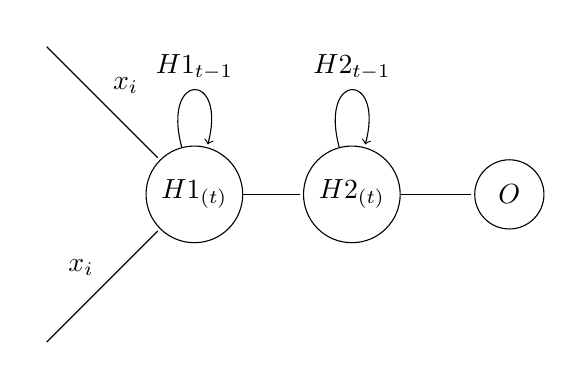
\begin{tikzpicture}[shorten >= 1pt, node distance = 2cm, on grid, auto, square/.style={regular polygon, regular polygon sides = 4}]
	\node[](0){};
	\node[below of = 0](1){};
	\node[below of = 1] (2){};
	
	\node[state, right of = 1](N1){$H1_{(t)}$};
	\node[state, right of = N1](N2){$H2_{(t)}$};
	\node[state, right of = N2](output){$O$};
	
	\draw[-]   (0) edge node{$x_i$}(N1)
	(2) edge node{$x_i$} (N1)
	(N1) edge[loop above] node{$H1_{t-1}$} (N1)
	(N2) edge[loop above] node{$H2_{t-1}$} (N2)
	(N1) edge (N2)
	(N2) edge (output);	
\end{tikzpicture}
\begin{center}
Iteration number 2 $t=2$
\end{center}
    \caption{A simplified representation of a node in a Reoccurrent Neural Network}\label{fig:rnn_neuron}
    
\end{figure}

% LSTM might be waaay too much detail. Also fuck its a *masive over-simplificatin*

For some particular tasks such as Natural language generation this setup is not enough, since as time goes on the network will develop a bias towards features present in more recent iteration; the influence of data from the older iteration will degrade over time, and the system will slowly tend to 'forget' features and patterns it learned at the beginnning: when it is then presented with new data it has never seen before, thi bias can pose a problem.

To dampen the effects of this bias one might employ Long-Short Term Memory cells (LSTM), a special kind on RNN neuron which can dynamically rank new information (and by extention, the content of its state) based on its relevance. LSTM ensures that important data is retained regardless on when it was learned, and thus diminishes the effect of the base RNN bias.\newline
It should be noted however that LSTM does not constitute a straight upgrade from the plain RNN architecture: it may be beneficial in certain cases, but decremental in others.
%maybe add a picture of a RNN or normal network for context?

\section{Generative Adversarial Networks} 

\cleardoublepage
\section{Experimental notes}
When training PassGAN on the libero set, the samples generates seem to have the genral pattern of user passwords; the network tries to generate strings that look like italian words, but are not. Testing of the output has not been performed yet, but i do wonder if including natural language dictionarie can help the network generate grammatically correct words and phrases.

It is yet to be established how grammatically correct words may affet the cracking.

In the next test i will try and add NL dictionaries and see how it goes. 

My hope is that the network can retain the currect password characteristics, but imporve its ability to generate natural langage fragments. Perhaps trnaference learning might come in handy for this?

\cleardoublepage
\thispagestyle{empty}
\printbibliography    
\end{document}
